\section{Anatomy of Standard Strategies}
\label{sec:eval-common-strategies}

In order to construct new baselines and their performance differences,
we evaluated tiebreaking strategies for domain-independent optimal
classical planning.  In our experiments, all planners are based on Fast
Downward, and all experiments are run with a 5-minute,
4GB memory limit for the search binary (FD translation/preprocessing
times are not included in the 5-minute limit).  All experiments were
conducted on Xeon E5410@2.33GHz CPUs. 

% following paragraph is added in order to avoid repeating the list of domains not
% included due to no coverage difference.
We used 1104 instances from 35 standard benchmark domains. These
instances are those originally included in the test suite of Fast
Downward planning system. In detail, they are: airport(50),
barman-opt11(20), blocks(35), cybersec(19), depot(22), driverlog(20),
elevators-opt11(20), floortile-opt11(20), freecell(80), grid(5),
gripper(20), hanoi(30), logistics00(28), miconic(150), mprime(35),
mystery(30), nomystery-opt11(20), openstacks-opt11(20),
parcprinter-opt11(20), parking-opt11(20), pathways(30),
pegsol-opt11(20), pipesworld-notankage(50), pipesworld-tankage(50),
psr-small(50), rovers(40), scanalyzer-opt11(20), sokoban-opt11(20),
storage(30), tidybot-opt11(20), tpp(30), transport-opt11(20),
visitall-opt11(20), woodworking-opt11(20), zenotravel(20).

\subsection{Does Last-Resort Strategies Make a Difference?}

We first compared two commonly used tiebreaking strategies, $[f,h,\fifo]$, $[f,h,\lifo]$, which
first break ties according to $h$, and then apply \fifo or \lifo
last-resort tiebreaking, respectively.
Results for LMcut heuristic \cite{Helmert2009} and M\&S heuristic \cite{HelmertHHN14} are
shown in \reftbl{tbl:lmcut-ipc-full} and \reftbl{tbl:mands-ipc-full}
(leftmost 2 columns), respectively.
Differences in coverage are observed in several domains, and
$[f,h,\lifo]$ outperforms $[f,h,\fifo]$ overall.

\begin{table}[htbp]
 {
 \centering
 \begin{center}
\begin{tabular}{|c|cccHHH|cccHHH|}
\hline
Domain & \([f,\fifo]\) & \([f,\lifo]\) & \([f,\ro]\) & R25103 & R4668 & R6506 & \([f,h,\fifo]\) & \([f,h,\lifo]\) & \([f,h,\ro]\) & lmh\(_{\text{R25103}}\) & lmh\(_{\text{R4668}}\) & lmh\(_{\text{R6506}}\)\\
\hline
IPC benchmark (1104) & 443 & \textbf{558} & 450 \(\pm\) 1 & 449 & 451 & 450 & 558 & \textbf{565} & 560.7 \(\pm\) 0.6 & 561 & 560 & 561\\
\hline
airport(50) & 18 & \textbf{26} & 18 & 18 & 18 & 18 & 27 & 26 & 26 & 26 & 26 & 26\\
barman-opt11(20) & 0 & 0 & 0 & 0 & 0 & 0 & 0 & 0 & 0 & 0 & 0 & 0\\
blocks(35) & 26 & 26 & 26 & 26 & 26 & 26 & 28 & 28 & 28 & 28 & 28 & 28\\
\textbf{cybersec(19)} & 0 & \textbf{3} & 0 & 0 & 0 & 0 & 2 & 3 & \textbf{4.3} \(\pm\) 0.6 & 4 & 5 & 4\\
depot(22) & 5 & 5 & 5 & 5 & 5 & 5 & 6 & 6 & 6 & 6 & 6 & 6\\
driverlog(20) & 12 & 13 & 12 & 12 & 12 & 12 & 13 & 13 & 13 & 13 & 13 & 13\\
elevators-opt11(20) & 14 & 15 & 14 & 14 & 14 & 14 & 15 & 15 & 15 & 15 & 15 & 15\\
floortile-opt11(20) & 6 & 6 & 6 & 6 & 6 & 6 & 6 & 6 & 6 & 6 & 6 & 6\\
freecell(80) & 8 & 9 & 9 & 9 & 9 & 9 & 9 & 9 & 9 & 9 & 9 & 9\\
grid(5) & 1 & 1 & 1 & 1 & 1 & 1 & 1 & 1 & 1 & 1 & 1 & 1\\
gripper(20) & 6 & 6 & 6 & 6 & 6 & 6 & 6 & 6 & 6 & 6 & 6 & 6\\
hanoi(30) & 12 & 12 & 12 & 12 & 12 & 12 & 12 & 12 & 12 & 12 & 12 & 12\\
logistics00(28) & 16 & \textbf{18} & 16 & 16 & 16 & 16 & 20 & 20 & 20 & 20 & 20 & 20\\
miconic(150) & 68 & \textbf{140} & 68 & 68 & 68 & 68 & 140 & 140 & 140 & 140 & 140 & 140\\
mprime(35) & 20 & 22 & 20 & 20 & 20 & 20 & 21 & 21 & 21 & 21 & 21 & 21\\
mystery(30) & 15 & 16 & 15 & 15 & 15 & 15 & 16 & 16 & 15.7 \(\pm\) 0.6 & 16 & 15 & 16\\
nomystery-opt11(20) & 12 & 13 & 12 & 12 & 12 & 12 & 14 & 14 & 14 & 14 & 14 & 14\\
\textbf{openstacks-opt11(20)} & 11 & \textbf{18} & 11.3 \(\pm\) 0.6 & 11 & 12 & 11 & 11 & \textbf{18} & 12 & 12 & 12 & 12\\
parcprinter-opt11(20) & 12 & 13 & 12 & 12 & 12 & 12 & 13 & 13 & 13 & 13 & 13 & 13\\
parking-opt11(20) & 1 & 1 & 1 & 1 & 1 & 1 & 1 & 1 & 1 & 1 & 1 & 1\\
pathways(30) & 4 & 5 & 4 & 4 & 4 & 4 & 5 & 5 & 5 & 5 & 5 & 5\\
pegsol-opt11(20) & 17 & 17 & 17 & 17 & 17 & 17 & 17 & 17 & 17 & 17 & 17 & 17\\
pipesworld-notankage(50) & 13 & 13 & 13 & 13 & 13 & 13 & 14 & 14 & 14.7 \(\pm\) 0.6 & 15 & 14 & 15\\
pipesworld-tankage(50) & 7 & 8 & 8 & 8 & 8 & 8 & 8 & 8 & 8 & 8 & 8 & 8\\
psr-small(50) & 48 & 48 & 48 & 48 & 48 & 48 & 48 & 48 & 48 & 48 & 48 & 48\\
rovers(40) & 7 & 7 & 7 & 7 & 7 & 7 & 7 & 7 & 7 & 7 & 7 & 7\\
scanalyzer-opt11(20) & 4 & \textbf{10} & 5.7 \(\pm\) 0.6 & 5 & 6 & 6 & 10 & 10 & 10 & 10 & 10 & 10\\
sokoban-opt11(20) & 19 & 19 & 19 & 19 & 19 & 19 & 19 & 19 & 19 & 19 & 19 & 19\\
storage(30) & 14 & 14 & 14 & 14 & 14 & 14 & 14 & 14 & 14 & 14 & 14 & 14\\
tidybot-opt11(20) & 11 & 12 & 11 & 11 & 11 & 11 & 12 & 12 & 12 & 12 & 12 & 12\\
tpp(30) & 6 & 6 & 6 & 6 & 6 & 6 & 6 & 6 & 6 & 6 & 6 & 6\\
transport-opt11(20) & 6 & 6 & 6 & 6 & 6 & 6 & 6 & 6 & 6 & 6 & 6 & 6\\
visitall-opt11(20) & 9 & 10 & 9.7 \(\pm\) 0.6 & 10 & 9 & 10 & 10 & 10 & 10 & 10 & 10 & 10\\
woodworking-opt11(20) & 6 & 9 & 8.3 \(\pm\) 0.6 & 8 & 9 & 8 & 10 & 10 & 10 & 10 & 10 & 10\\
zenotravel(20) & 9 & \textbf{11} & 9 & 9 & 9 & 9 & 11 & 11 & 11 & 11 & 11 & 11\\
\hline
\end{tabular}
\end{center}

 % \begin{tabular}{|*{5}{c|}}
\hline
 & \multicolumn{4}{|c|}{Coverages (\# problems solved)} \\
\hline                                    
 Domain                                 &  $[f,h,\fifo]$ &  $[f,h,\lifo]$ &  $[f,\fifo]$ &  $[f,\lifo]$ \\ \hline
 sum(1104)                              &558             &\textbf{565}    &442           &556           \\ \hline
 {\relsize{-1}airport(50)}              &\textbf{27}     &26              &18            &26            \\
 {\relsize{-1}barman-opt11(20)}         &0               &0               &0             &0             \\
 {\relsize{-1}blocks(35)}               &\textbf{28}     &\textbf{28}     &26            &26            \\
 {\relsize{-1}cybersec(19)}             &2               &\textbf{3}      &0             &\textbf{3}    \\
 {\relsize{-1}depot(22)}                &\textbf{6}      &\textbf{6}      &5             &5             \\
 {\relsize{-1}driverlog(20)}            &13              &13              &12            &13            \\
 {\relsize{-1}elevators-opt11(20)}      &15              &15              &14            &15            \\
 {\relsize{-1}floortile-opt11(20)}      &6               &6               &6             &6             \\
 {\relsize{-1}freecell(80)}             &9               &9               &8             &9             \\
 {\relsize{-1}grid(5)}                  &1               &1               &1             &1             \\
 {\relsize{-1}gripper(20)}              &6               &6               &6             &6             \\
 {\relsize{-1}hanoi(30)}                &12              &12              &12            &12            \\
 {\relsize{-1}logistics00(28)}          &\textbf{20}     &\textbf{20}     &16            &18            \\
 {\relsize{-1}miconic(150)}             &\textbf{140}    &\textbf{140}    &68            &\textbf{140}  \\
 {\relsize{-1}mprime(35)}               &21              &21              &19            &\textbf{22}   \\
 {\relsize{-1}mystery(30)}              &15              &16              &15            &15            \\
 {\relsize{-1}nomystery-opt11(20)}      &\textbf{14}     &\textbf{14}     &12            &13            \\
 {\relsize{-1}openstacks-opt11(20)}     &11              &\textbf{18}     &11            &\textbf{18}   \\
 {\relsize{-1}parcprinter-opt11(20)}    &13              &13              &12            &13            \\
 {\relsize{-1}parking-opt11(20)}        &1               &1               &1             &1             \\
 {\relsize{-1}pathways(30)}             &5               &5               &4             &5             \\
 {\relsize{-1}pegsol-opt11(20)}         &17              &17              &17            &17            \\
 {\relsize{-1}pipesworld-notankage(50)} &\textbf{15}     &14              &13            &13            \\
 {\relsize{-1}pipesworld-tankage(50)}   &8               &8               &7             &8             \\
 {\relsize{-1}psr-small(50)}            &48              &48              &48            &48            \\
 {\relsize{-1}rovers(40)}               &7               &7               &7             &7             \\
 {\relsize{-1}scanalyzer-opt11(20)}     &\textbf{10}     &\textbf{10}     &4             &\textbf{10}   \\
 {\relsize{-1}sokoban-opt11(20)}        &19              &19              &19            &19            \\
 {\relsize{-1}storage(30)}              &14              &14              &14            &14            \\
 {\relsize{-1}tidybot-opt11(20)}        &12              &12              &11            &11            \\
 {\relsize{-1}tpp(30)}                  &6               &6               &6             &6             \\
 {\relsize{-1}transport-opt11(20)}      &6               &6               &6             &6             \\
 {\relsize{-1}visitall-opt11(20)}       &10              &10              &9             &10            \\
 {\relsize{-1}woodworking-opt11(20)}    &\textbf{10}     &\textbf{10}     &6             &9             \\
 {\relsize{-1}zenotravel(20)}           &\textbf{11}     &\textbf{11}     &9             &\textbf{11}   \\\hline
\end{tabular}

 \caption{
 Coverage comparison (the number of instances solved in 5min, 2GB, LMcut
 heuristics) between
 the standard baseline tiebreaking algorithms. We highlight the
 best results when the difference between the maximum and the mininum coverage exceeds 2.
 }
 \label{tbl:lmcut-ipc-full}
 }
\end{table}

\begin{table}[htbp]
 {
 \centering
 \begin{center}
\begin{tabular}{|c|cccHHH|cccHHH|}
\hline
Domain & \([f,\fifo]\) & \([f,\lifo]\) & \([f,\ro]\) & R25103 & R4668 & R6506 & \([f,h,\fifo]\) & \([f,h,\lifo]\) & \([f,h,\ro]\) & lmh\(_{\text{R25103}}\) & lmh\(_{\text{R4668}}\) & lmh\(_{\text{R6506}}\)\\
\hline
IPC benchmark (1104) & 460 & 490 & 462 \(\pm\) 2 & 464 & 462 & 460 & 491 & 496 & 490 \(\pm\) 1 & 491 & 490 & 489\\
\hline
airport(50) & 9 & 9 & 9 & 9 & 9 & 9 & 9 & 9 & 9 & 9 & 9 & 9\\
barman-opt11(20) & 4 & 4 & 4 & 4 & 4 & 4 & 4 & 4 & 4 & 4 & 4 & 4\\
blocks(35) & 21 & 22 & 21 & 21 & 21 & 21 & 22 & 22 & 22 & 22 & 22 & 22\\
\textbf{cybersec(19)} & 0 & 0 & 0 & 0 & 0 & 0 & 0 & 0 & 0 & 0 & 0 & 0\\
depot(22) & 5 & 6 & 5 & 5 & 5 & 5 & 6 & 6 & 5 & 5 & 5 & 5\\
driverlog(20) & 12 & 12 & 12 & 12 & 12 & 12 & 12 & 12 & 12 & 12 & 12 & 12\\
elevators-opt11(20) & 13 & 13 & 13 & 13 & 13 & 13 & 13 & 13 & 13 & 13 & 13 & 13\\
floortile-opt11(20) & 5 & 6 & 5 & 5 & 5 & 5 & 6 & 6 & 6 & 6 & 6 & 6\\
freecell(80) & 15 & 16 & 15 & 15 & 15 & 15 & 17 & 17 & 16 & 16 & 16 & 16\\
grid(5) & 2 & 2 & 2 & 2 & 2 & 2 & 2 & 2 & 2 & 2 & 2 & 2\\
gripper(20) & 8 & 20 & 8 & 8 & 8 & 8 & 20 & 20 & 20 & 20 & 20 & 20\\
hanoi(30) & 14 & 14 & 14 & 14 & 14 & 14 & 14 & 14 & 14 & 14 & 14 & 14\\
logistics00(28) & 20 & 20 & 20 & 20 & 20 & 20 & 20 & 20 & 20 & 20 & 20 & 20\\
miconic(150) & 68 & 73 & 68.7 \(\pm\) 1.2 & 70 & 68 & 68 & 73 & 73 & 73.3 \(\pm\) 0.6 & 73 & 73 & 74\\
mprime(35) & 23 & 23 & 22.3 \(\pm\) 0.6 & 22 & 22 & 23 & 23 & 24 & 23.7 \(\pm\) 0.6 & 24 & 23 & 24\\
mystery(30) & 15 & 15 & 15 & 15 & 15 & 15 & 15 & 16 & 15 & 15 & 15 & 15\\
nomystery-opt11(20) & 17 & 18 & 18 & 18 & 18 & 18 & 18 & 18 & 18 & 18 & 18 & 18\\
\textbf{openstacks-opt11(20)} & 15 & 19 & 15.7 \(\pm\) 0.6 & 16 & 16 & 15 & 15 & 19 & 15.7 \(\pm\) 0.6 & 16 & 16 & 15\\
parcprinter-opt11(20) & 10 & 10 & 10 & 10 & 10 & 10 & 10 & 10 & 10 & 10 & 10 & 10\\
parking-opt11(20) & 1 & 1 & 1 & 1 & 1 & 1 & 1 & 1 & 1 & 1 & 1 & 1\\
pathways(30) & 4 & 4 & 4 & 4 & 4 & 4 & 4 & 4 & 4 & 4 & 4 & 4\\
pegsol-opt11(20) & 17 & 19 & 17.3 \(\pm\) 0.6 & 17 & 18 & 17 & 19 & 19 & 19 & 19 & 19 & 19\\
pipesworld-notankage(50) & 9 & 9 & 8.7 \(\pm\) 0.6 & 9 & 9 & 8 & 10 & 10 & 9.7 \(\pm\) 0.6 & 10 & 10 & 9\\
pipesworld-tankage(50) & 13 & 13 & 13.3 \(\pm\) 0.6 & 14 & 13 & 13 & 13 & 13 & 13.7 \(\pm\) 0.6 & 14 & 14 & 13\\
psr-small(50) & 50 & 50 & 50 & 50 & 50 & 50 & 50 & 50 & 50 & 50 & 50 & 50\\
rovers(40) & 6 & 8 & 6 & 6 & 6 & 6 & 8 & 8 & 8 & 8 & 8 & 8\\
scanalyzer-opt11(20) & 10 & 10 & 10 & 10 & 10 & 10 & 10 & 10 & 10 & 10 & 10 & 10\\
sokoban-opt11(20) & 20 & 20 & 20 & 20 & 20 & 20 & 20 & 20 & 20 & 20 & 20 & 20\\
storage(30) & 15 & 15 & 15 & 15 & 15 & 15 & 15 & 15 & 15 & 15 & 15 & 15\\
tidybot-opt11(20) & 0 & 0 & 0 & 0 & 0 & 0 & 0 & 0 & 0 & 0 & 0 & 0\\
tpp(30) & 6 & 6 & 6 & 6 & 6 & 6 & 7 & 6 & 6 & 6 & 6 & 6\\
transport-opt11(20) & 7 & 7 & 7 & 7 & 7 & 7 & 7 & 7 & 7 & 7 & 7 & 7\\
visitall-opt11(20) & 9 & 9 & 9 & 9 & 9 & 9 & 9 & 9 & 9 & 9 & 9 & 9\\
woodworking-opt11(20) & 7 & 7 & 7 & 7 & 7 & 7 & 7 & 7 & 7 & 7 & 7 & 7\\
zenotravel(20) & 10 & 10 & 10 & 10 & 10 & 10 & 12 & 12 & 12 & 12 & 12 & 12\\
\hline
\end{tabular}
\end{center}

 % \begin{tabular}{|*{5}{c|}}
\hline
                                        & \multicolumn{4}{|c|}{Coverages (\# problems solved)}  \\ \hline                                    
 Domain                                 &  $[f,h,\fifo]$ &  $[f,h,\lifo]$ &  $[f,\fifo]$ &  $[f,\lifo]$ \\ \hline                                    
 sum(1104)                              &479           &\textbf{488}  &451         &481         \\ \hline                                    
 {\relsize{-1}airport(50)}              &9             &9             &9           &8           \\
 % {\relsize{-1}barman-opt11(20)}         &4             &4             &4           &4           \\
 {\relsize{-1}blocks(35)}               &22            &21            &21          &21          \\
 % {\relsize{-1}cybersec(19)}             &0             &0             &0           &0           \\
 {\relsize{-1}depot(22)}                &5             &6             &5           &5           \\
 {\relsize{-1}driverlog(20)}            &12            &12            &11          &12          \\
 {\relsize{-1}elevators-opt11(20)}      &12            &12            &11          &11          \\
 {\relsize{-1}floortile-opt11(20)}      &6             &6             &5           &5           \\
 {\relsize{-1}freecell(80)}             &\textbf{17}   &\textbf{17}   &15          &16          \\
 % {\relsize{-1}grid(5)}                  &2             &2             &2           &2           \\
 {\relsize{-1}gripper(20)}              &\textbf{20}   &\textbf{20}   &7           &\textbf{20} \\
 % {\relsize{-1}hanoi(30)}                &14            &14            &14          &14          \\
 % {\relsize{-1}logistics00(28)}          &20            &20            &20          &20          \\
 {\relsize{-1}miconic(150)}             &\textbf{73}   &\textbf{73}   &68          &72          \\
 {\relsize{-1}mprime(35)}               &23            &24            &23          &23          \\
 {\relsize{-1}mystery(30)}              &15            &16            &15          &15          \\
 {\relsize{-1}nomystery-opt11(20)}      &18            &18            &17          &18          \\
 {\relsize{-1}openstacks-opt11(20)}     &13            &\textbf{19}   &13          &\textbf{19} \\
 {\relsize{-1}parcprinter-opt11(20)}    &9             &9             &10          &10          \\
 % {\relsize{-1}parking-opt11(20)}        &1             &1             &1           &1           \\
 % {\relsize{-1}pathways(30)}             &4             &4             &4           &4           \\
 {\relsize{-1}pegsol-opt11(20)}         &\textbf{19}   &\textbf{19}   &17          &\textbf{19} \\
 {\relsize{-1}pipesworld-notankage(50)} &8             &9             &8           &8           \\
 % {\relsize{-1}pipesworld-tankage(50)}   &13            &13            &13          &13          \\
 % {\relsize{-1}psr-small(50)}            &50            &50            &50          &50          \\
 {\relsize{-1}rovers(40)}               &\textbf{8}    &\textbf{8}    &6           &\textbf{8}  \\
 % {\relsize{-1}scanalyzer-opt11(20)}     &10            &10            &10          &10          \\
 {\relsize{-1}sokoban-opt11(20)}        &19            &19            &19          &20          \\
 % {\relsize{-1}storage(30)}              &15            &15            &15          &15          \\
 % {\relsize{-1}tidybot-opt11(20)}        &0             &0             &0           &0           \\
 % {\relsize{-1}tpp(30)}                  &6             &6             &6           &6           \\
 % {\relsize{-1}transport-opt11(20)}      &6             &6             &6           &6           \\
 % {\relsize{-1}visitall-opt11(20)}       &9             &9             &9           &9           \\
 % {\relsize{-1}woodworking-opt11(20)}    &7             &7             &7           &7           \\
 % {\relsize{-1}zenotravel(20)}           &10            &10            &10          &10          \\
\hline
\end{tabular}

 \caption{
 Coverage comparison (the number of instances solved in 5min, 2GB, M\&S heuristics) between
 the standard baseline tiebreaking algorithms. We highlight the
 best results when the difference between the maximum and the mininum coverage exceeds 2.
 }
 \label{tbl:mands-ipc-full}
 }
\end{table}

\subsection{Is $h$-Based Tiebreaking Necessary?}

\label{sec:h-necessary}

In the right half of \reftbl{tbl:lmcut-ipc-full} and
\reftbl{tbl:mands-ipc-full}, we show the results of $[f, \fifo]$ and
$[f, \lifo]$, the \astar variants which rely on \fifo or \lifo
last-resort tiebreaking only.  $[f,\lifo]$, which simply breaks ties
among nodes with the same $f$-cost by expanding the most recently
generated nodes first \cite{korf1985depth}, clearly dominates
$[f,\fifo]$.  Interestingly, the performance of the $[f,\lifo]$ strategy
is comparable to $[f,h,\lifo]$ and $[f,h,\fifo]$, and it even dominates
$[f,h,\fifo]$ in Openstacks.
% the standard two-level strategies that first break ties according to $h$.
This may be surprising, considering the ubiquity of $h$-based tiebreaking in the search and planning communities.

\lifo behaves somewhat similarly to $h$-based tiebreaking, in the following sense:
\lifo expands the most recently generated node $n$.
For any child $n'$, 
if the heuristic function is admissible and $f(n') = f(n)$, there are only 2 possibilities :
(1) $g(n') > g(n)$ and $h(n') < h(n)$, or
(2) $g(n') = g(n)$ and $h(n') = h(n)$,
because $g(n)+h(n)=g(n')+h(n')$.
Thus, as \lifo expands nodes in a ``depth-first'' manner,
the nodes that continue to be expanded in the plateau by \lifo have non-increasing $h$-values,
much like in $h$-based tiebreaking.
Although the expansion order of $[f,\lifo]$ is not strictly the same as that of $h$-based tiebreaking strategies,
this explains their similarity in performances.

% \textbf{An in-depth investigation of the behavior of $[f,\lifo]$ vs. $h$-based tiebreaking is a direction for future work.}
% Compared to the $h$-based variants which explicitly selects nodes with smaller $h$ and its expanded nodes have non-increasing $h$-values,
% This has the same  can behave somewhat similarly to actively expanding nodes with low $h$-values, as done by $h$-based tiebreaking.
% \citeauthor{burns2012implementing}
% (\citeyear{burns2012implementing}) writes ``the goal can be found more
% quickly in the final $f$ layer of search'' about $h$ tiebreaking.

\subsection{Plateaus and Tiebreaking}

\refig{fig:f-h-eval} gives us a
more fine-grained analysis by comparing the number of node evaluation
(computations of \lmcut) in each instance between $[f,h,\lifo]$ and $[f,h,\fifo]$ strategies.
It shows that the difference in the number of nodes
evaluated can sometimes be larger than a factor of 10 (\pddl{Openstacks}, \pddl{Cybersec} domains).
Contrarly to the conventional wisdom, 
these results suggest that last-resort tiebreaking can have a significant effect on
the search performance.

\begin{figure}[htbp]
 \centering \relsize{-3}
 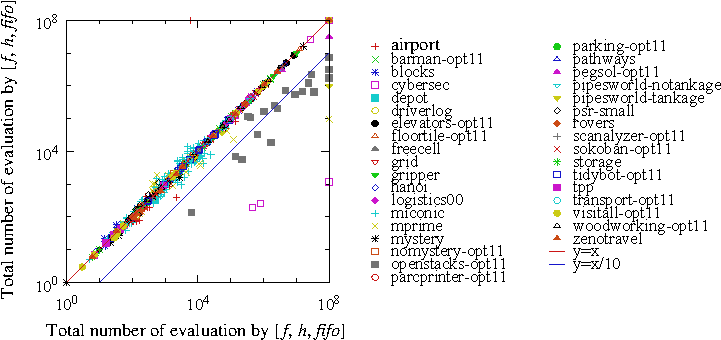
\includegraphics{tables/aaai16-30min-5min-cut/aaai16prelim3/evaluated-lmcut_ff-lmcut_lf.pdf}
 \caption{The number of LMcut evaluations on various planning domains,
 with standard \fifo vs \lifo last-resort tiebreaking, both with $h$
 tiebreaking. \lifo evaluates  less than $1/10$ of the nodes evaluated
 by \fifo in \pddl{Cybersec} and \pddl{Openstacks}. 
 }
 \label{fig:f-h-eval}
\end{figure}

% In a plateau, the heuristics do not provide any useful guidance -- a
% plateau region requires a blind search because all neighboring nodes have the same
% estimates. Because of this, search algorithms rely solely on the tiebreaking criterion.

% We further investigate the cause of this performance difference in detail.

A natural but false assumption behind this conventional wisdom would be as follows.
% 
First, the effect of the last-resort tiebreaking strategies (\lifo or
\fifo) under the presence of $h$-tiebreaking is
limited to the search plateau $\plateau{f,h}$, the set of nodes which
share the same $f$ values and $h$ values.
% 
Also, in optimal search, the two \astar with
different last-resort tiebreaking strategies both search the same set of
nodes in the region where $f<f^*$.
% 
% If $h$-tiebreaking is enabled, the two \astar variants also expands the same number of nodes with $h>0$.
Furthermore, the nodes with $h>0$ never become the goal nodes when $h$ is admissible.
% 
Therefore, the effect of last-resort tiebreaking is limited to
the final plateau $\plateau{f^*,0}$.
% 
With all these constraints, the region should sound very small compared to the
total size of the search space required to be expanded by \astar.

However, counter-intuitively, such a region can be so large enough to
cause a performance difference, or it can even account for \emph{most} of the
search effort required by \astar.
\refig{fig:plateau} plots the size of this final plateau on 1104 IPC
benchmark instances.  The $y$-axis represents the number of nodes with
$f=f^*, h=0$, the final plateau, and the $x$-axis represents the total
number of nodes expanded so far. This figure suggests that, in some
domains such as \pddl{Openstacks} and \pddl{Cybersec}, the planner
spends most of the runtime searching the final plateau for a solution,
even with the help of $h$ tiebreaking.

\begin{figure}[htbp]
   \centering
  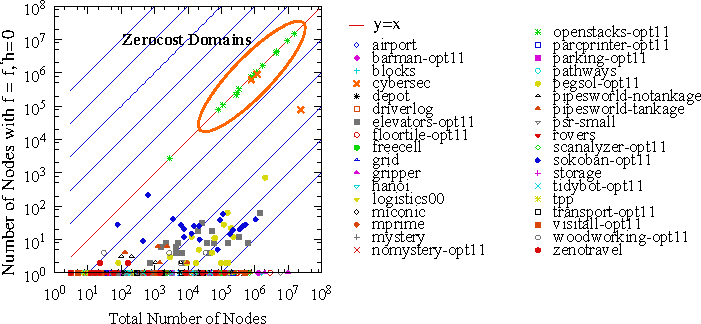
\includegraphics{tables/aaai16-frontier/aaai16prelim3/lmcut_frontier-front.pdf}
  \caption{
 The number of nodes with $f=f^*, h=0$ (y-axis), which form
  the final plateau when $h$-based tiebreaking is enabled, compared to
  the total number of nodes in the search space (x-axis) with $f\leq
  f^*$ on 1104 IPC benchmark problems.  Note that \pddl{Openstacks}
  and \pddl{Cybersec} instances are near the $y=x$ line.
  This statistics is obtained by running a modified Fast Downward with
 \lmcut which continues searching after the solution is found
 until expanding all nodes with cost $f=f^*$.} \label{fig:plateau}
\end{figure}


A natural question might be that what makes these two domains,
\pddl{Openstacks} and \pddl{Cybersec}, different from all other domains
which have much smaller final plateaus.
